\documentclass{article}

\usepackage{amsmath}
\usepackage{mathtools}
\usepackage{amstext}
\usepackage{array}
\usepackage[long]{optidef}
\usepackage[backend=biber,
            url=false]{biblatex}
\usepackage{float}
\usepackage{tikz}
\usepackage{txfonts}
\usepackage[colorinlistoftodos]{todonotes}
\usepackage[long]{optidef}

  \addbibresource{ch1-2.bib}

  \usetikzlibrary{calc,matrix,decorations.markings,decorations.pathreplacing}
  \usetikzlibrary{positioning}

  \definecolor{colone}{gray}{0.7}
  \definecolor{coltwo}{gray}{0.6}
  \definecolor{colthree}{gray}{0.5}
  \definecolor{colfour}{gray}{0.9}
  \definecolor{colfive}{gray}{0.9}
  \definecolor{colsix}{gray}{0.9}
  \definecolor{colseven}{gray}{0.9}

  \tikzset{
  table/.style={
  matrix of nodes,
  row sep=-\pgflinewidth,
  column sep=-\pgflinewidth,
  nodes={rectangle,text width=2cm,align=center},
  text depth=1.25ex,
  text height=2.5ex,
  nodes in empty cells}
  }

  \tikzstyle{startstop} = [rectangle, minimum width=2cm, minimum height=1.5cm,text centered, draw=black]
  \tikzstyle{process} = [rectangle, minimum width=3cm, minimum height=1.5cm, text centered, draw=black]
  \tikzstyle{blank} = [circle, minimum width=0.1cm, minimum height=0.1cm, text centered, draw=white]
  \tikzstyle{arrow} = [thick,->,>=stealth]

\begin{document}

  \title{Chapter 2}

  \author{M. Repetto}

  \date{}

\maketitle

\begin{abstract}
  In the following paper is proposed a multi-objective model for components allocation in a Green Supply Chain framework. The model builds on the concept of the supply chain as suggested by Porter, and accounts for the costs of production using the Activity Based Cost accounting method (ABC). Such model is organized in blocks related to several moments in the value chain, from the procurement to the end customer. Above each and every one of these blocks, a series of environmental constraints have been included, and that the firm has to comply, with respect to specific country regulation, or in case of a particular Corporate Environmental Responsibility policy...\todo{to be continued when the model will be fully defined}
\end{abstract}

\section{Introduction}
  Global Supply Chain Management (GSCM) is probably one of the most used terms when the discussion of how the firms are running their business is brought to the table nowadays. GSCM may be defined as the allocation of goods and services along a series of transnational companies' global network to maximize profits and minimize waste. As the Supply Chain Professionals puts it, the goal of GSCM is threefold and focuses on delivering: (a)the right product; (b)to the right place; (c)at the right time.
  Inside this very wide paradigm, the concept of logistics serves as the backbone; recalling that logistics is developed to be in charge of the movement of goods, service and last but not least information from the sourcing of raw material, till it reaches the end customer.
  Along with these two concepts a third one sticks with them, the Green Supply Chain (GSC). This idea, brought to light by a more advanced concern about environmental matters of the developed countries, forced the firms to be accountable for their negative externalities related to the environment in which they operate \cite{srivastava_green_2007}.

  However such legislation lacks from a point of view of legal constraints, setting only a few qualitative restriction, poorly measurable by the enterprises or in some cases letting the customers pay for their environmental behavior toward waste disposition. These facts are inevitably leaving some degrees of freedom to the firms, on the other hand, is also important to notice that these are only seeds of legislation that show us how the long-term trend will be about the tolerance given to the behavior of firms with environmental concerns, a trend that in the future may require firms to set particular frameworks to be accountable for their environmental impact. Nowadays such effort is not achieved by the legal frameworks provided by the domestic legislators but by the Corporate Environmental Responsibility (CER), meaning that are the stakeholders to impose the companies to be more responsible on their day to day operations.

  Speaking about the literature, is observable an emerging branch which deals with the Green Supply Chain Management, a new paradigm of Supply Chain Management whose aim is to keep under control the behavior of the firm during its operations, by applying policies such as Green Manufacturing and Re-manufacturing, Green Design etc... Because of that a Goal Programming model is proposed, in order to address such problems; following what proposed by literature, an enhanced model is proposed, such model, fixing quantitative and qualitative constraints to the pollution generated by the value adding activities, involved in the creation of the good, tries to implement the benefits of a recycling program enacted by the firm apropos the WEEE directive. In the case under scope, the choice was to pick a networking electronic appliance business (i.e. hub, switch or router).  In order to measure such impact, a framework provided by the Activity Based Costing is used; such approach is used in order to assess and address the marginal environmental impact of any additional unit elaborated by the transnational firms.
\\
\\
The paper is organized in four parts where two of them are devoted to a review of the existing literature and the last two, which are a respectively model and result oriented. In the first of the literature sections a full overview of the Green Supply Chain framework will be given; at the same time the focus will be directed to the legal implications that are affecting both producer and distributors operating in the European Union. After this overview a deep analysis will be given on the state-of-the-art techniques used to model both Supply Chain Management and Logistics topics, focusing the attention on peculiar applications such as stochastic programming. Ultimately the two sections devoted to the model will be used to state the model proposed with its assumptions, and then to analyze its result through a scenario analysis.  


\pagebreak

\section{Green Supply Chain}
Green Supply Chain saw a steady growth of interest in many enterprises\cite{Diabat2011} as well as by academics; a growth that, looking to the data\cite{Strobel18}, reached its hype between the 2012 and 2014 (Figure \ref{fig:occurrence}) and that may be strengthen in the next years because of the increasing environmental concern. The main research fields interested by this phenomena are the ones involving environmental sciences, management, operational research and more generally green sustainable sciences\cite{Shan2018}  
\begin{figure}[ht]
	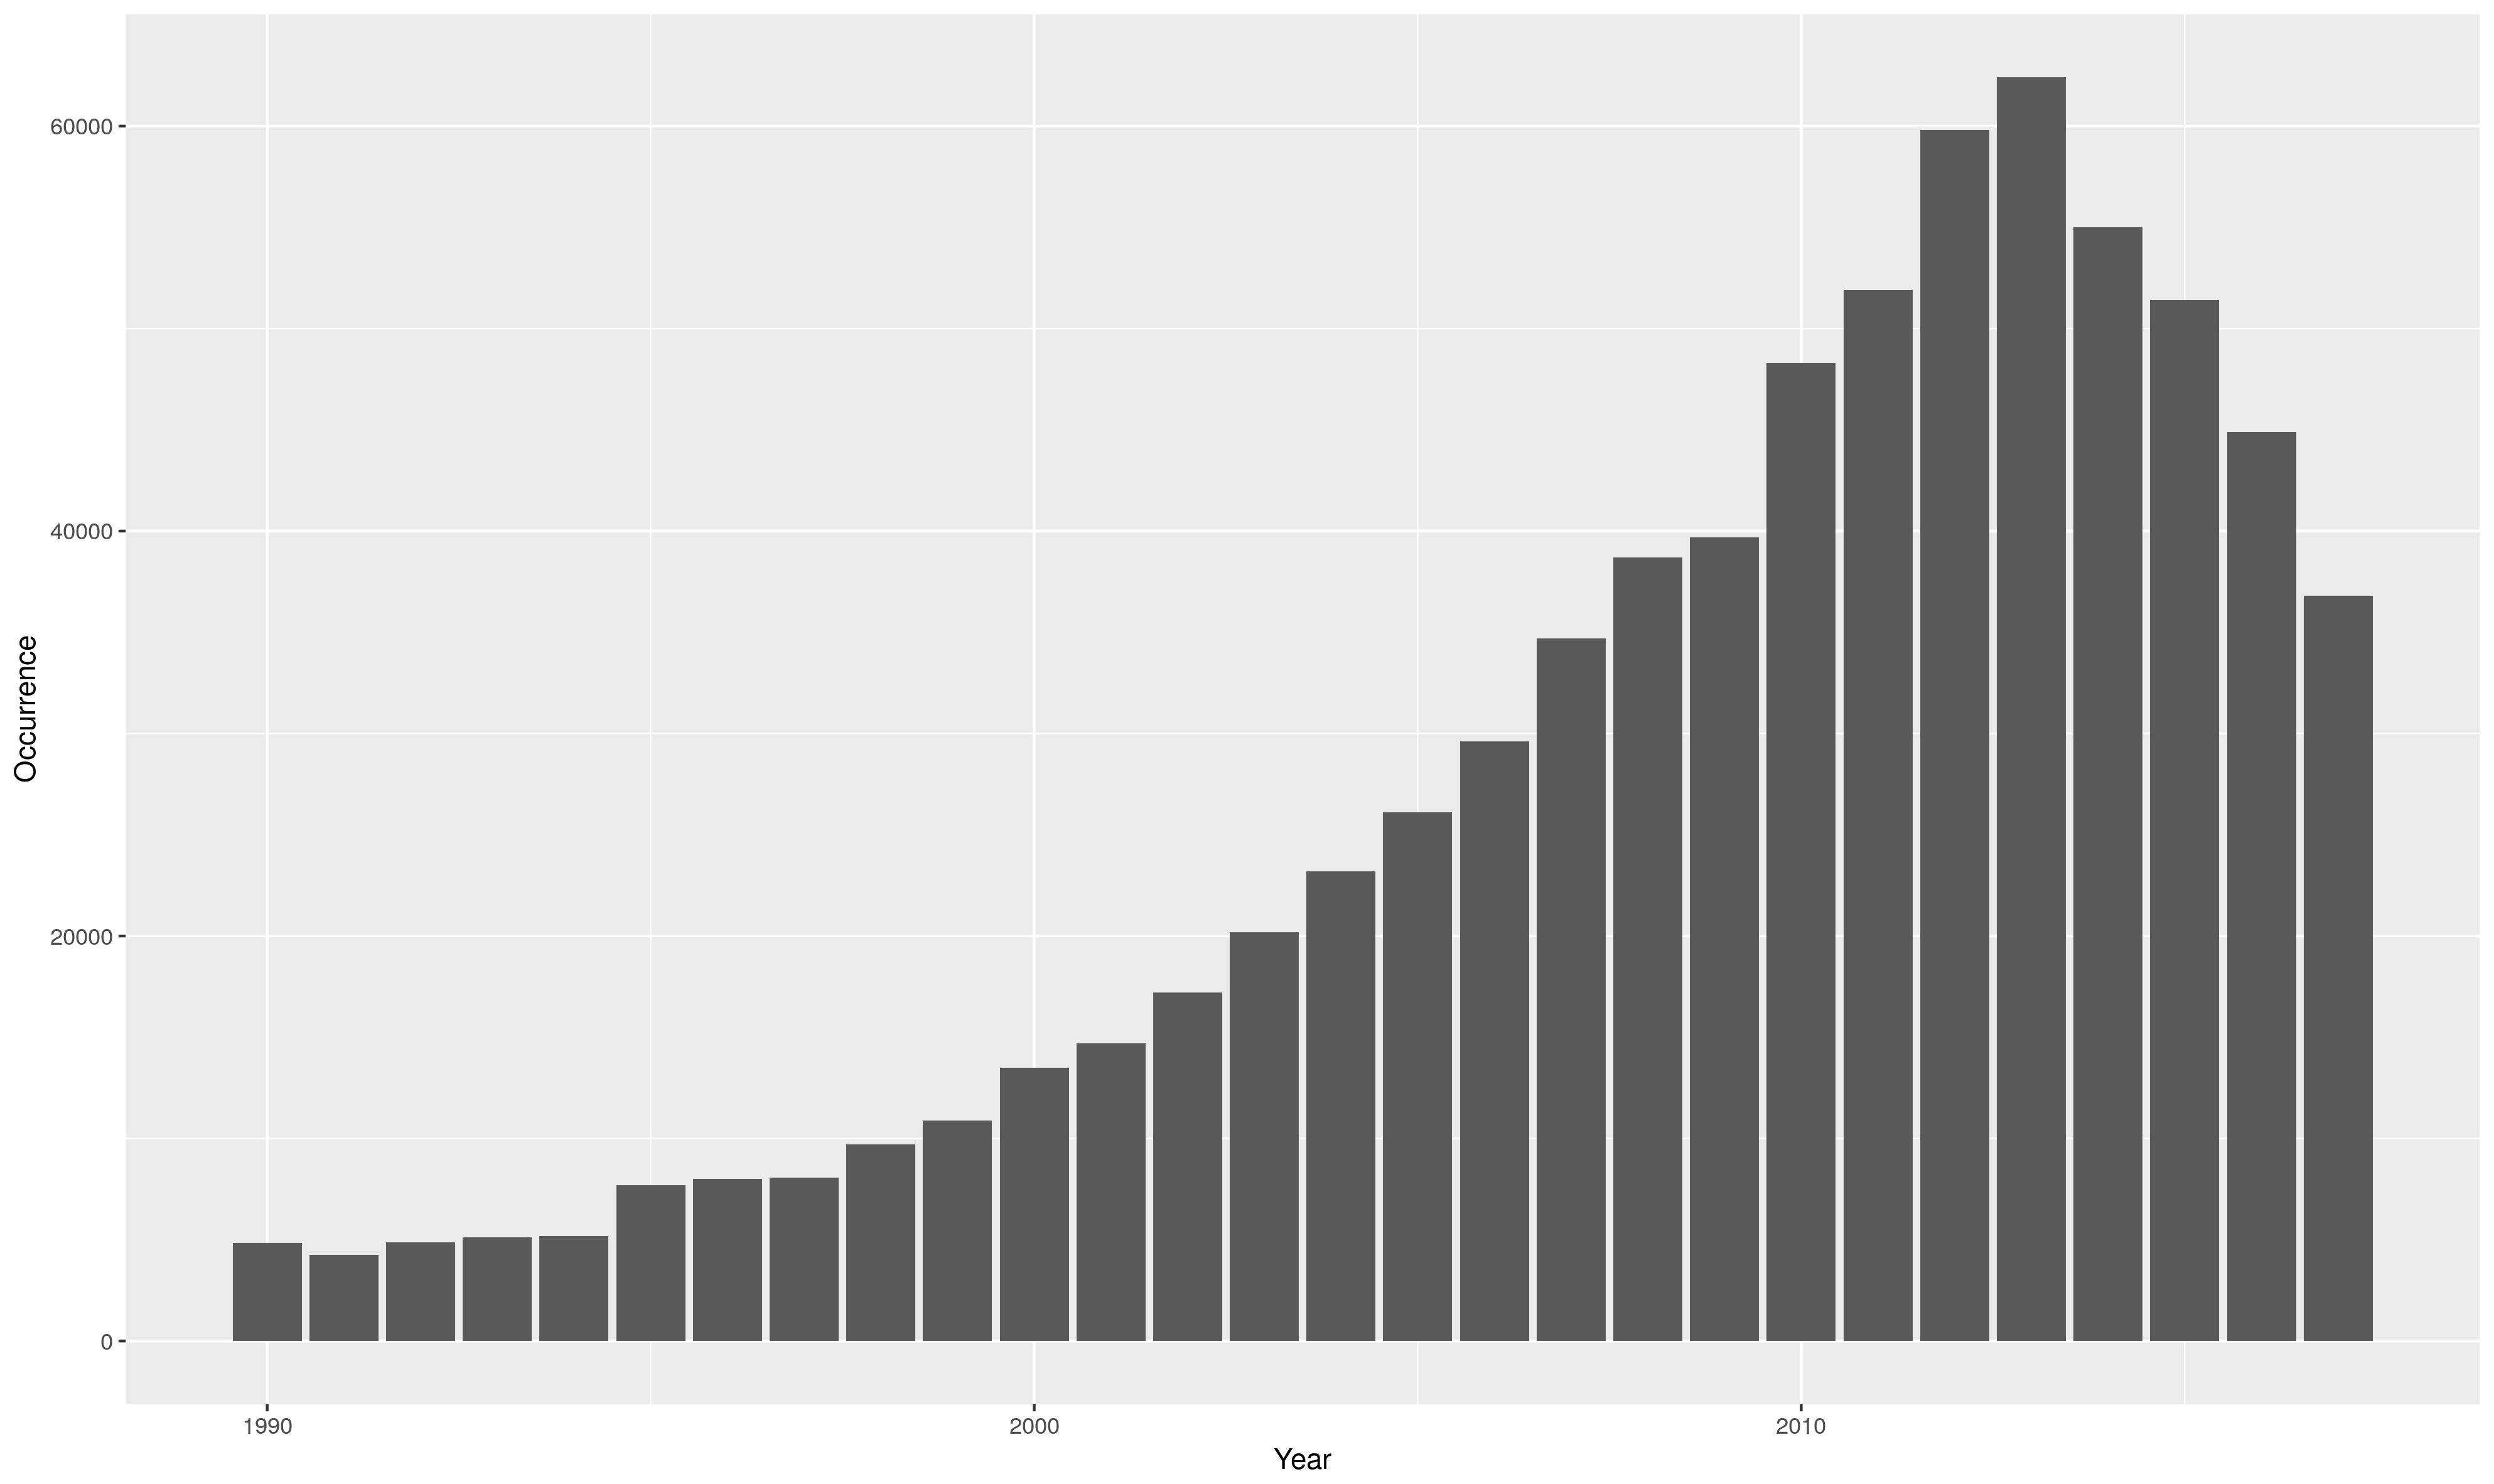
\includegraphics[width=\textwidth]{Images/occurence.png}	
	\label{fig:occurrence}
	\caption{Occurrence of Green Supply Chain in papers indexed by Google Scholar}	
\end{figure}
\\
Although Green Supply Chain manager is perceived as a game changer in order to unleash long term sustainability of a business, it's worth noting the lack of an univocal definition. In fact, some of the academics see GSCM as a process\cite{Gilbert2001}, more specifically a "greening process" from this school of thought belongs the line of thought that the management has the duty of incorporating the environmental criteria along all the organizational value creation process. Another definition sees the Green Supply Chain as a set of policies whose focus is to raise environmental concern along the production, distribution process\cite{Zsidisin2001}. In this paper we used a two level definition the first definition is a formal one that builds from the concept of Supply Chain Management as defined by the Council of Supply Chain Management Professionals; the second is a substantial and deals with the operations affecting the "green" practices inside the firm.
\\
In formal terms, Green Supply Chain may be defined as the series of interconnected activities across the border of different enterprises that adds value to the goods and services from the sourcing to the market. Its aim is to improve performance in measures of sustainability, cost reduction, emission reduction. Whereas Supply Chain Management sets its objectives to maximize profits and minimize waste, in economic terms, Green Supply Chain sets its objectives even further, posing as its ultimate mission to lower the ecological impact that a firm or a series of them has in their day to day operations. 
Such green operations\cite{srivastava_green_2007}\cite{Zhu2008} constitutes the substantial definition of Green Supply Chain Management, these operations are:
  \begin{itemize}
    \item Green Manufacturing and Re-manufacturing: is the process of controlling and reutilizing material in the manufacturing, in order to limit waste creation\cite{urvashi_green_2013};
    \item Green Design: is an approach put in place to promote the environmental quality of a certain product or service,  by reducing negative impacts on the natural environment; an example could be the automatic switch of the television after a period of idleness\cite{ceschin_evolution_2016}; and
    \item Green Operations in general: by green operation is intended any type of activity which does not fall into the two categories mentioned above but is characterized by a "green" attitude as for example the optimization of the offices consumption through a remote-working policy;
  \end{itemize}
  
  Apart from the definition and its importance in the business field is important to focus the attention of the main drivers affecting this change, in fact such drivers are many and involves the overall ecosystem of the firm (external drivers), and even the firm (internal drivers) in its reactions to this drivers plays a key role in setting its environmental behavior that may be reactive, focused, opportunistic, and proactive\cite{YolLee2007}. Speaking about the external drivers, they fall between four main categories:
  \begin{itemize}
	  \item Legal frameworks: embraces all the set of laws either soft or hard laws, that implies certain standards and regulation over the operations provided along the supply chain;
	  \item Customer relations and concerns: in this category pertain every possible action overtaken by the end-users who can force their pressure on the firm enacting non buying campaign and manifestation in general;
	  \item Supplier/distributors relations: the actions pertaining to this category are similar to the ones of the customers, the only difference is that since are enacted    by entities that are constituting the supply chain they can provoke major issue in providing good and services on the market;
	  \item External stakeholders, this category embraces all the stakeholders that do not follow in the categories of either customers and suppliers, which may include stockholder, agents involved by the environmental behavior of the firm, is an example the households living near the production plan, etc...
  \end{itemize}
Since the model proposed has it's aim in setting a Green Supply Chain network of products from the procurement sites to the end user market which has stated to be the Euro Zone; it's necessary to highlight the set of norms that characterizes such market and in particular a specific attention will be given to the norms concerning electrical products.

  \subsection{The legal framework: an European perspective}
  In the market under scope which is the European one, there are several legislation concerning the environmental impact of certain e-Products\footnote{for e-Products, is intended an electrical or electronic equipment such as computers, TV-sets, fridges, cell phones and other electronic appliances}. The most important are:
  \begin{itemize}
    \item Waste Electrical \& Electronic Equipment (WEEE);
    \item Restriction on Hazardous Substances (RoHS);and
    \item Ecodesign Requirement for Energy-using Product (EuP).
  \end{itemize}

  Such legal frameworks act at different levels from the sourcing to the customer involving community member States. The following flowchart illustrates this differences.

  \begin{figure}[ht]
    \centering

    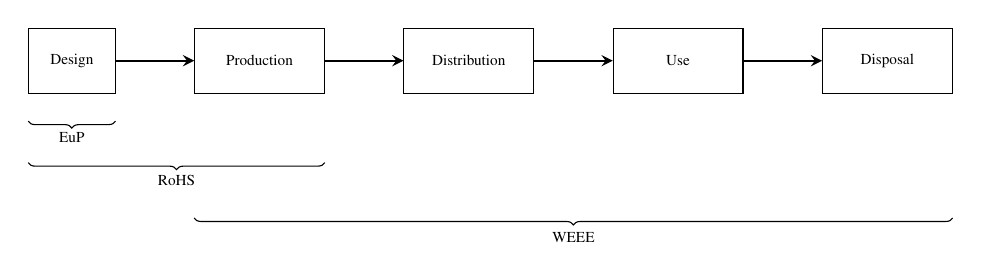
\begin{tikzpicture}[scale=0.8, every node/.style={scale=0.55}]
    \node (start) [startstop] {Design};
    \node (process1) [process, right=of start] {Production};
    \node (process2) [process, right=of process1] {Distribution};
    \node (process3) [process, right=of process2] {Use};
    \node (process4) [process, right=of process3] {Disposal};

    \draw [arrow] (start)--(process1);
    \draw [arrow] (process1)--(process2);
    \draw [arrow] (process2)--(process3);
    \draw [arrow] (process3)--(process4);

    \draw[decorate,decoration={brace,mirror,raise=10pt}]
    (start.south west) -- (start.south east) node[below, midway, yshift = -22]  {EuP};
    \draw[decorate,decoration={brace,mirror,raise=25pt}]
    (start.south west) -- (process1.south east) node[below, midway, yshift = -50]  {RoHS};
    \draw[decorate,decoration={brace,mirror,raise=45pt}]
    (process1.south west) -- (process4.south east) node[below, midway, yshift = -88]  {WEEE};

    \end{tikzpicture}
    \caption{Legislation affection}
  \end{figure}

  In the following subsection, an additional overview is given to such legislation.

\subsubsection{Waste Electrical \& Electronic Equipment}
  The Waste Electrical \& Electronic Equipment also called WEEE is ruled in the European Community by Directive 2002/96/EC now repealed by the Directive 2012/19/EU. The objectives of the policy are, to preserve, protect and improve the quality of the environment, to protect human health and to utilize natural resources prudently and rationally. That policy is based on the precautionary principle meaning that the polluter should pay for its damage. Is important to notice that in the European market such directive is impacting all the community members is not perfectly homogeneous ways because of the implementation which is remitted to the local authorities. This problem may incur in potential elusive behavior as highlighted by the German firms who exploited gaps in the law which have allowed them to move large amounts of WEEE declared for recycling to developing economies including India, China, Nigeria and Eastern Europe \cite{ongondo_how_2011}. Despite such cases, the overall impact of this directive is mostly positive as highlighted by the Eurostat data here exposed.

  The WEEE Directive currently sets a minimum collection target of 4 kg per year per inhabitant for WEEE from households. From 2016, the minimum collection rate shall be 45\% calculated on the basis of the total weight of WEEE collected. Where the WEEE is calculated with the following formula:
  $$
  W (n) = \sum{t = t_0}_{n} POM \cdot L^p(t,n)
  $$
  Where $W(n)$ refers to the specific quantity of electrical and electronic waste for a specific year, $POM(n)$ is the quantity of new electrical component injected in the market and $L$ is the discard-based lifespan profile for the electrical component injected in the market. From the graph proposed below is possible to see how the target of minimum collection of 4 kg per year per inhabitant for WEEE from households was achieved by all the countries in the Euro zone however not all the countries has the same collection rate, meaning that some of them may have introduced legislation that comply only with the minimum target of the directive, leaving the households with the freedom to dispose of their WEEE in unconventional manner. Clearly this means for the enterprises less obligations on the collection of e-Products, but at the same time less products to be recycled and less opportunity of remanufacturing.

  \begin{figure}
  \centering
  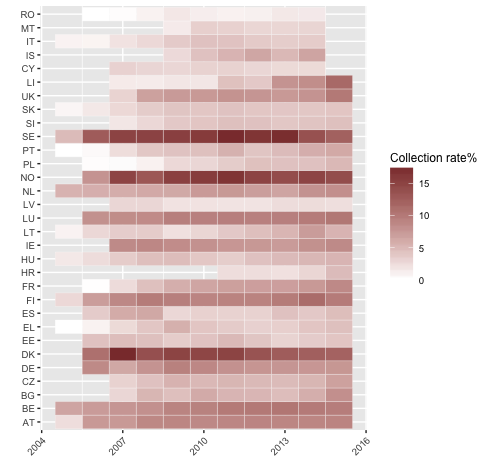
\includegraphics[width=0.8\linewidth]{Images/heatmap.png}
  \caption{Kilograms of WEEE collected per capita}
  \end{figure}

\subsubsection{Restriction on Hazardous Substances}
  The Restriction on Hazardous Substances also called RoHS is represented by the Directive 2017/2102 (RoHS 2 recast). The scope is the restriction on the use of certain hazardous substances in electrical and electronic equipment (EEE) such as lead, mercury, cadmium, hexavalent chromium etc... In such case, as opposed to the WEEE the RoHS directive acts as a barrier to the products containing such minerals and not when they become waste. In considering such regulation is worth noting that there are no differences between the dimension of the distributing entity, meaning that small businesses, as well as large businesses, are equally affected by these restrictions. The only amendment is given to the batteries that may exceed such restriction.

\subsubsection{Ecodesign Requirements for Energy-using Product}
  The Directive 2009/125/EC is meant to deal with Ecodesign regulations. Ecodesign regulations require manufacturers to decrease the energy consumption of their products by establishing minimum energy efficiency standards. In particular, The Ecodesign Directive provides a consistent legal framework for improving the environmental performance of products setting out a minimum mandatory requirement for the energy efficiency of these products. In case of the design of IT networking products such as routers and switches the firms are obliged by such directive to implement some ecodesign features such as the maximum wattage of 1W in case of off mode or a standby maximum consumption of 2W. Such measure per se do not impact in any case the supply chain since they are just additional features that has to be implemented in the products sold in Europe.

\pagebreak 

\section{A state-of-the-art review: mathematical modeling in SCM}
  As proposed by the Council of Supply Chain Management Professionals, the Supply Chain Management (SCM) is the planning and the management of all activities involved in sourcing and procurement, conversion, and logistics as well as coordination and collaboration with the entities. The problem arising from such activities seems to be well addressed by mathematical modeling, other advantages of such approach are the economic sustainability and the possibility to scale the model in order to address different situations.
  From the comprehensive review built by Muna et al. \cite{mula_mathematical_2010} the methods used by the academic world and the specific situations they tried to model, are:
  \begin{itemize}
	  \item Linear Programming: order quantity definition by means of decentralization\cite{jung_order_2008}, production and distribution planning taking into account country specific regulations\cite{Oh_Karimi_2006}, multiple points of sales planning\cite{Kanyalkar_2005};
	  \item Mixed Integer Linear Programming: network optimization and routing configuration\cite{romo_optimizing_2009}, distribution planning in an environment with just a production plant and many distribution centers\cite{Rizk_Martel2008};
    \item Non Linear Programming: optimization of production, transport and inventories\cite{benjamin_analysis_1989};
    \item Multi Objective Programming: replenishment production and distribution planning with conflicting objectives simultaneously\cite{torabi_interactive_2008}, master planning\cite{Chern_Hsieh_2007};
    \item Fuzzy Mathematical Programming: distribution allocation considering different products and production/distribution centers\cite{Liang_Cheng_2009};
    \item Stochastic Programming: addressing demand uncertainty accounting for the probability distribution\cite{Gupta_Maranas_2003};
    \item Heuristics Algorithms and Meta-Heuristics; and
    \item Hybrid Models.
  \end{itemize}

  Is worth noting how the majority of the models pertain to the category of Mixed Integer Linear Programming, this may be due to the fact that is probably one of the simplest and most reliable methods that can be used to solve such problems, however, this simplicity comes with some costs such as the focus on a single linear objective function with linear constraints whereas in reality different objectives has to be taken into account as for example the manager preferences toward greener choices. Another interesting topic brought into light by Aouni \cite{azimian_supply_2017} is that such models are generally deterministic, where in reality such assumption does not hold most of the time, for example, the demand forecast can't be deterministic at all and derives from a stochastic process. This lack of deterministic variable lies also in case of the procurement where the price of a commodity is said to follow a sort of stochastic process and an order may be placed several days after the decision make it. Both of these situations, namely the fuzziness of the DM and the stochastic process of the demand will be modeled using two variances from the plain vanilla GP, that are stochastic Goal Programming and Fuzzy Goal Programming. 

  \subsection{Stochastic Optimization: a Goal Programming perspective}
  As previously stated, deterministic models seems to be the preferred choice by practitioners and academics whereas in reality there's a certain level of uncertainty that comes into play when deciding over the setting of supply chain. When a decision maker is facing a multitude of random objectives is stated to face a multi objective stochastic program (MSP). Because of it's flexibility Goal Programming turned to be a very powerful tool in modeling multi objective deterministic problem. The formulation originally proposed by Charnes and Cooper\cite{charnes_optimal_1955} was built for deterministic scenarios, and with further development, starting from Contini\cite{Contini1968}, a newer branch was developed which accounted for non deterministic situations, namely stochastic Goal Programming. The resulting model is generalized as follow:
\begin{mini!}
	{\tilde{\delta^+},\tilde{\delta^-}}{\sum_{i=i}^{N}\tilde{\delta^+_i} +\tilde{\delta^-_i}}{}{}
	\addConstraint{f_i(x)-\tilde{\delta^+_i}+\tilde{\delta^+_i}}{=\tilde{g_i},}{\forall i \in N}
	\addConstraint{x\in h_s(x)}{\leq 0}{\forall s \in M}
	\addConstraint{\tilde{\delta^+},\tilde{\delta^-}}{\geq 0}{}
\end{mini!}
Where the goal variable $\tilde{g}$ is said to follow a certain probability distribution. A very common solution to deal with such stochastic problem is transform the undeterministic problem into a deterministic one (also called deterministic equivalent formulation). Looking at the general formulation made before, if $\tilde{g}$(or the $\tilde{g_i}$ vector in our case) is said to follow a normal distribution $N(\mu;\sigma^2)$, therefore we can reformulate the program in its equivalent formulation\cite{azimian_supply_2017} 
\begin{mini!}
	{\tilde{\delta^+},\tilde{\delta^-}}{\sum_{i=i}^{N}\tilde{\delta^+_i} +\tilde{\delta^-_i}}{}{}
	\addConstraint{f_i(x)-\tilde{\delta^+_i}+\tilde{\delta^+_i}}{=\mu_i,}{\forall i \in N}
	\addConstraint{x\in h_s(x)}{\leq 0}{\forall s \in M}
	\addConstraint{\tilde{\delta^+},\tilde{\delta^-}}{\geq 0}{}
\end{mini!}

  \subsection{Fuzzy Goal Programming}
  Fuzzy GP is a subset of Goal Programming models that uses fuzzy sets, which were firstly developed by Zadeh\cite{Zadeh_1965}. The main advantage of fuzzy sets is that they can better model the level of imprecision of a particular feature of the model, usually such imprecision deals with the target goal, but this do not mean that fuzzy target goals are the only factors that can be enhanced via fuzzy sets. The fundamental part of a fuzzy GP is the membership function (or in case of multiple fuzzy sets, functions)characterizing the shape of the fuzzy sets, and also how it penalizes values above and below some predetermined thresholds. In fuzzy GP the most common membership functions used are: (1) right-sided, used to penalize positive deviations; (2)left sided, used to penalize negative deviations; (3) triangular shaped, in this case the membership function penalizes both positive and negative deviations;(4) trapezoidal shaped, similar to the triangular shaped, since both positive and negative deviations are penalized, however in this case we allow for an interval of complete satisfaction.
  Recent works of fuzzy GP were made in the field of engineering where fuzzy sets where used to model the perfect selection of wind turbine in order to fully unleash the potential of each particular sites\cite{Rehman2017}; in the field of management, where a case study of wastewater treatment was proposed, combining both fuzzy GP and Stochastic GP\cite{Diaz-Madronero2018}; and in the field of social sciences where fuzzy GP was applied in analyzing environmental and sustainability goals of a country spotting improvement opportunities, requirement of efforts and implementing the sustainable development plans\cite{Nomani2016}.  
  \pagebreak

\section{Model formulation}
The hybrid model developed is based on the supply chain concept developed by Santoso\cite{Santoso_Ahmed_Goetschalckx_Shapiro_2005}plus the integration of supporting activities as enunciated by Porter\cite{CompetitiveAdvantage}in his concept of value chain. Apart from these features, as the model is built with the concept of Green Supply Chain management seemed necessary to enhance the basic capabilities of a open loop supply chain network with the characteristics of a typical reverse supply chain network (which is intended to be in closed loop fashion). Because of the reverse supply chain network a series of new entities have been introduced, namely the recollection points, which in our case are the same retail stores, and the recycling point that has to comply both with regulation and with management expectation in terms of recycled products. Therefore, a fuzzy goal is created using the fuzzy goal programming formulation developed by the \cite{YAGHOOBI2008}, such formulation, as reported previously, tries to capture the DM preferences about units recycled and the bottom line imposed by regulations.
\subsection{Open Loop Supply Chain}
In a very general open loop supply chain model the materials after been purchased pass through a series of entities where the material is transformed into goods (operation activities), then follows the process of outbound logistics when the goods produced has to reach their specific market for satisfying consumer demand, however such last operation is subject to certain cost, such as the sales force and marketing campaigns which are, generally, managed and supervised by the national retail stores in each specific country.
A general formulation of such model is given by Santoso and is formulated as follows:
\begin{mini!}
	{y,x}{\sum_{i=1}^{P} c_i y_i  + \sum_{k=1}^{K} \sum_{(i,j)=1,1}^{A} q_{ij}^{k}x_{ij}^{k}}{}{}
	\addConstraint{\sum_{i=1}^{N} x_{ij}^k - \sum_{l=1}^{N} x_{jl}^k}{=0,}{\forall j \in P, \forall k \in K}
	\addConstraint{\sum_{i=1}^{N} x_{ij}^k}{\geq d_{j}^k,}{\forall j \in C, \forall k \in K}
\addConstraint{\sum_{j=1}^{N} x_{ij}^{k}}{\leq s_{i}^{k},}{\forall i \in L, \forall k \in K}
	\addConstraint{\sum_{k=i}^{K} r_{j}^k \cdot \sum_{i=1}^{N}x_{ij}^k}{\leq m_j y_i,}{\forall j \in P}
	\addConstraint{x \in \varmathbb{R}^+}{y \in Y[0,1]}{}
\end{mini!}

Where the objective function $(3a)$ is to minimize both the variable and fixed costs (here represented by the cost of building a plant) of a particular supply chain network.
The constraint posed in $(3b)$ serves to maintain the flow constant in each passage(so called flow conservation) it serves to balance the net inflow with the net outflow; the second and third constraint here represented by $(3c)$ and $(3d)$ are respectively controlling the volume of the demand (receiver side) and the supply (supplier side) of the supply chain network; whereas the fourth constraint $(3e)$ is used to control the capacity of each node. Lastly, the $x$ variable, indicating the flow of goods has to be positive and the variable $y$ indicating the effective construction of the plant to assume value that is either 1 or 0, in other terms $y$ is said to be binary. 
\\
However the model is complete from a point of view of supply chain modeling it's worth noting that such model do not implement any support activities, whereas the Porter model mentions them. Therefore the hybrid model will contain a set of constraint indicating such activities and a new objective function embracing this change.

\begin{figure}[ht]
  \centering

  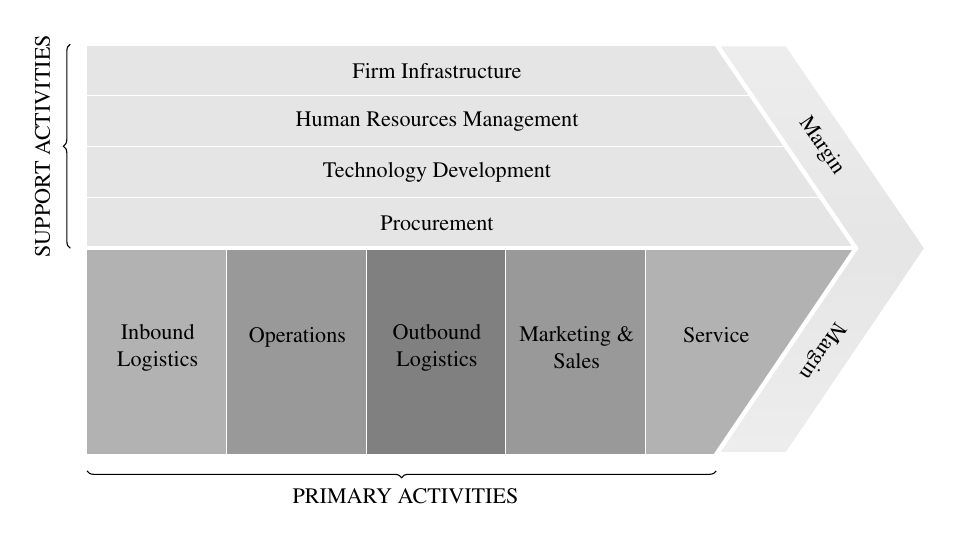
\begin{tikzpicture}[scale=0.8, every node/.style={scale=0.8}]
  \matrix (mat) [table]
  {
  |[fill=colfour]| & |[fill=colfour]| & |[fill=colfour]| & |[fill=colfour]| & |[fill=colfour]| &  \\
  |[fill=colfive]| & |[fill=colfive]| & |[fill=colfive]| & |[fill=colfive]| & |[fill=colfive]| &  \\
  |[fill=colsix]| & |[fill=colsix]| & |[fill=colsix]| & |[fill=colsix]| & |[fill=colsix]| & |[fill=colsix]| \\
  |[fill=colseven]| & |[fill=colseven]| & |[fill=colseven]| & |[fill=colseven]| & |[fill=colseven]| & |[fill=colseven]| \\
  |[fill=colone]| & |[fill=coltwo]| & |[fill=colthree]| & |[fill=coltwo]| & |[fill=colone]| & |[fill=colone]|  \\
  |[fill=colone]| & |[fill=coltwo]| & |[fill=colthree]| & |[fill=coltwo]| & |[fill=colone]| & |[fill=colone]|  \\
  |[fill=colone]| & |[fill=coltwo]| & |[fill=colthree]| & |[fill=coltwo]| & |[fill=colone]| & \\
  |[fill=colone]| & |[fill=coltwo]| & |[fill=colthree]| & |[fill=coltwo]| & |[fill=colone]| &  \\
  };

  \foreach \row in {2,3,4}
  \draw[white] (mat-\row-1.north west) -- (mat-\row-6.north east);
  \draw[white,ultra thick] (mat-1-1.north west) -- (mat-1-6.north east);
  \draw[white,ultra thick] (mat-5-1.north west) -- (mat-5-6.north east);

  \foreach \col in {2,3,4,5}
  \draw[white] (mat-5-\col.north west) -- (mat-8-\col.south west);

  \node[fill=colfour] at (mat-1-3) {Firm Infrastructure};
  \node[fill=colfive] at (mat-2-3) {Human Resources Management};
  \node[fill=colsix] at (mat-3-3) {Technology Development};
  \node[fill=colseven] at (mat-4-3) {Procurement};
  \node at ([yshift=-10pt]mat-6-1) {\parbox[t]{2cm}{\centering Inbound Logistics}};
  \node at ([yshift=-10pt]mat-6-2) {\parbox[t]{2cm}{\centering Operations \\\mbox{}}};
  \node at ([yshift=-10pt]mat-6-3) {\parbox[t]{2cm}{\centering Outbound Logistics}};
  \node at ([yshift=-10pt]mat-6-4) {\parbox[t]{2cm}{\centering Marketing \& Sales}};
  \node at ([yshift=-10pt]mat-6-5) {\parbox[t]{2cm}{\centering Service \\\mbox{}}};
  \node[rotate = 90] at ([xshift=-52pt]mat-3-1.north) {SUPPORT ACTIVITIES};
  \node at ([yshift=-19pt,xshift=-0.5cm]mat-8-3.south) {PRIMARY ACTIVITIES};

  \fill[white] (mat-1-5.north east) -- (mat-5-6.north east) -- (mat-1-6.north east) -- cycle;
  \fill[white] (mat-8-5.north east) -- (mat-5-6.north east) -- (mat-8-6.north east) -- cycle;

  \shade[top color=colfour!70,bottom color=colfour!70,middle color=colseven,draw=white,ultra thick]
  (mat-1-5.north) -- (mat-5-6.north) -- (mat-8-5.south) --
  (mat-8-5.south east) -- (mat-5-6.north east) -- (mat-8-5.south east) --
  (mat-5-6.north east) -- (mat-1-5.north east) -- cycle;

  \begin{scope}[decoration={markings,mark=at position .5 with \node[transform shape] {Margin};}]
  \path[postaction={decorate}]
  ( $ (mat-1-5.north)!0.5!(mat-1-5.north east) $ ) -- ( $ (mat-5-6.north)!0.5!(mat-5-6.north east) $ );
  \path[postaction={decorate}]
  ( $ (mat-5-6.north)!0.5!(mat-5-6.north east) $ ) -- ( $ (mat-8-5.south)!0.5!(mat-8-5.south east) $ );
  \end{scope}

  \draw[decorate,decoration={brace,mirror,raise=6pt}]
  (mat-1-1.north west) -- (mat-5-1.north west);
  \draw[decorate,decoration={brace,mirror,raise=6pt}]
  (mat-8-1.south west) -- (mat-8-5.south);
  \end{tikzpicture}

  \caption{Porter's Value Chain}
\end{figure}

Such activities are a fundamental part on the supply chain that serves as glue with the supply chain steps to the deliver the value to the end-customer. Therefore the hybrid model should take them into account, a revised version then is proposed.

\begin{mini!}
  {x}{\sum_{k=1}^{K} \sum_{(i,j)=1,1}^{A} q_{ij}^{k}x_{ij}^{k} + \sum_{i=1}^{N} c_i \sum_{k=1}^{K} \sum_{(i,j)=1,1}^{A}x_{ij}^{k}}{}{}
  \addConstraint{\sum_{i=1}^{N} x_{ij}^k - \sum_{l=1}^{N} x_{jl}^k }{=0,}{\forall j \in P, \forall \in K}
  \addConstraint{\sum_{i=1}^{N} x_{ij}^k}{\geq d_{j}^k,}{\forall j \in C, \forall k \in K}
\addConstraint{\sum_{j=1}^{N} x_{ij}^{k}}{\leq s_{i}^{k},}{\forall i \in L, \forall k \in K}
\addConstraint{\sum_{k=i}^{K} r_{j}^k \cdot \sum_{i=1}^{N}x_{ij}^k }{\leq m_j,}{\forall j \in P}
\addConstraint{\sum_{i=1}^{N} q_{i}^j}{= n_j,}{\forall j \in P}
\addConstraint{x \in \varmathbb{R}^+ }{,}{}
\end{mini!}

In formulating our hybrid model is not taken into account the fixed cost of building a plant, this happened for two reasons. The first reason is the consideration of the cost of building a plant as a sunk cost and therefore it should not influence the economic decision on whether to allocate a particular quantity of goods on a specific plant. Secondly, the Activity Based Cost method is used therefore  the focus will be on the activities that contributes in creating the marginal cost of the good in the supply chain.

\subsection{Closed Loop Supply Chain}
In the previous sections a model of open loop was presented, however in green supply chain something as an open loop supply chain network do not exist, this is because of the after life treatment of the products selled by the company. Such procedure is also enforced by hard laws (as analyzed in the specific section). Therefore the revised model will have to capture these features. The closed loop supply chain network will be enunciated as follow:

\begin{mini!}
	{x}{\sum_{i=1}^{I}\sum_{j=1}^{J}\sum_{k=1}^{K} c^f_{ijk} x^f_{ijk}  + {\sum_{k=1}^{K}\sum_{l=1}^{L}\sum_{i=1}^{I0} c^r_{kli} x^r_{kli}}{}{}
	\addConstraint{\sum_{i=1}^{I}\sum_{j=1}^{J} x^f_{ijk}{= d_k,}{\forall k \in K}
	\addConstraint{\sum_{l=1}^{L}(\sum_{i=0}^{I} x^r_{kli} - x^r_{kli})}{= w_k,}{\forall k \in K}
	\addConstraint{\lambda \sum_{i=1}^{I0} x^r_{kli}}{\leq x^r_{il},}{\forall k \in K ,\forall l \in L}
	\addConstraint{\sum_{k=1}^{K} \sum_{i=1}^{L} r_k x^r_{kli}}{\leq \sum_{k=1}^{K} d_k,}{\forall i \in I}
	\addConstraint{x \in \varmathbb{R}^+ }{,}{}
\end{mini!}
The model enunciated minimizes two different flow costs, namely the one implying the forward flow, the one from the production plant to the consumer and the reverse flow that follows the opposite direction, namely from the consumer to the production plant passing thorugh ad-hoch dismantling plants. The constraints applied to such moodel are therefore a combination of both forward flow constraints, mitigated from the classical open loop supply chain, and the reverse flow constraints. The constraint at $1$ is stating that the forward flow must equal the demand of the costumer at a particular retailing site; where instead the constraint at $2$ is enunciating the amount of waste that will not be part of the recycling process. The constraint at $3$ focuses on imposing a threashold in which the units recycled will not be of any advantage for the production plan and therefore will constitute additional waste. Lastly constraint $4$ that states the inequality about the products collected that should not exceed the products delivered at a $k$ general retail store. 

The model presented however does not implement any decision maker preferences nor any legal boundaries on which the recycling center has to be submitted. Because the electronic waste turns out to be a resource for the firm is necessary to model the fuzziness of such desire expressed by the DM, and therefore the implementation of a Fuzzy set\cite{Zadeh_1965}, turns out to be the best choice; such set has a membership function defined as:
$$
\mu [f_k(x)]=
\begin{cases}
1 & f_k(x) \geq b_k \\
1-\frac{b_k-f_k(x)}{n_{max}} & b_k -n{max} \leq f_k(x) \leq b_k \\
0 & f_k(x) \leq b_k - n_{max}
\end{cases}
$$
The defined set penalizes the negative occurrences from the target demanded by the decision maker, and at the same time guarantees a bottom line coherent with the local legislation.

\subsection{The Goal Programming model}
Since the goals of the problem stated before are trying to model a set of different objectives the choices was to opt for the Goal Programming as a multi-criteria analysis tool therefore the resulting model will be set as follow: 
\\
The model proposed takes into account only one commodity because of simplicity matters however it can be adjusted to allow more than one commodity by including the transformation process of each production step. The additional rules to be implemented in the model may derive from other supply chain management tool more focused on the operational level such as production tree, etc... An example of such integration is proposed below.

In this case is possible to see how the two initial commodities are transformed passing through the production stage in one product that from now on will be used in the model for all the additional processes. From such simple example is evident that the process of transformation creates less goods passing from a stage to another, conversely the opposite contradict the production tree assumptions and therefore will not be taken into account. 

\subsubsection{Objective function}
The objective function that has to be minimized contains all the deviation from the soft constraints contained in equations ... 
\subsubsection{Soft Constraints}
The hard constraints identified by the equations from ... to ... are summarized below 
\subsubsection{Hard Constraints}

\subsubsection{Model formulation}

\begin{mini!}
  {x}{\sum_{k=1}^{K} \sum_{(i,j)=1,1}^{A} q_{ij}^{k}x_{ij}^{k} + \sum_{i=1}^{N} c_i \sum_{k=1}^{K} \sum_{(i,j)=1,1}^{A}x_{ij}^{k}}{}{}
  \addConstraint{\sum_{i=1}^{N} x_{ij}^k - \sum_{l=1}^{N} x_{jl}^k }{=0,}{\forall j \in P, \forall \in K}
  \addConstraint{\sum_{i=1}^{N} x_{ij}^k}{\geq d_{j}^k,}{\forall j \in C, \forall k \in K}
\addConstraint{\sum_{j=1}^{N} x_{ij}^{k}}{\leq s_{i}^{k},}{\forall i \in L, \forall k \in K}
\addConstraint{\sum_{k=i}^{K} r_{j}^k \cdot \sum_{i=1}^{N}x_{ij}^k }{\leq m_j,}{\forall j \in P}
\addConstraint{\sum_{i=1}^{N} q_{i}^j}{= n_j,}{\forall j \in P}
\addConstraint{x \in \varmathbb{R}^+ }{,}{}
\end{mini!}

\pagebreak

\section{Results and Conclusion}
The model was tested with the data exposed in the table below:

Even if the fuzzy membership functions for the recycling plants where assumed to be given, a sensitivity analysis of the wheights was performed. Such sensitivity analysis is proposed in an ad-hoc section. Addittionally a Analytical Hierarcical Process was run in order to assess the perfect wheight assessment. Then the model was solved using the NEOS servers throug the CPLEX solver. 

\subsection{Sensitivity analysis}

\subsection{Analytical Hierarcical Process for wheight determination}

\begin{itemize}
	\item
	\item
\end{itemize}


\newpage 

\printbibliography

\end{document}
